% SECTION: Expectation-Maximization (EM) Algorithmus
\section{Expectation-Maximization (EM) Algorithmus}

\divider

% SUBSECTION: Problemstellung
\subsection{Problemstellung}

% Problemstellung
\begin{frame}{Problemstellung}{}
	\begin{itemize}
		\item Wir betrachten ein statistisches Modell mit den Daten $\bX = \bigl( \bx_1, \bx_2, \ldots, \bx_N \bigr)^\top$,
			den \keyword{latenten Variablen} $\bZ = \bigl( \bz_1, \bz_2, \ldots, \bz_N \bigr)^\top$ und den Modellparametern $\btheta$.
		\item Wie üblich ist unser Ziel die Maximierung der Log-Likelihood $\ln p(\bX \param \btheta)$ bezüglich $\btheta$.
		\item Wir nehmen an, dass die gemeinsame Verteilung $p(\bX, \bZ \param \btheta)$ von $\bX$ und $\bZ$ gegeben ist.
		\item Hieraus können wir $\ln p(\bX \param \btheta)$ bestimmen, indem wir $\bZ$ \textit{marginalisieren}:
		\begin{equation} \label{eq:em-incomplete-log-likelihood}
			\ln p(\bX \param \btheta) = \ln \sum_{\bZ} p(\bX, \bZ \param \btheta)
		\end{equation}
		\item In der Regel ist eine direkte Maximierung von \eqref{eq:em-incomplete-log-likelihood} zu kompliziert,
			da der Logarithmus nicht direkt auf $p(\bX, \bZ \param \btheta)$ wirken kann.
	\end{itemize}
\end{frame}


% Problemstellung (Forts.)
\begin{frame}{Problemstellung (Forts.)}{}
	\begin{itemize}
		\item Mit $\{ \bX, \bZ \}$ bezeichnen wir den \keyword{vollständigen} Datensatz, $\bX$ alleine nennen wir hingegen \keyword{unvollständig}.
		\item Analog nennen wir $\ln p(\bX, \bZ \param \btheta)$ die \keyword{vollständige Log-Likelihood} und $\ln p(\bX \param \btheta)$ die
			\keyword{unvollständige Log-Likelihood}.
	\end{itemize}
\end{frame}


% Expectation-Maximization (EM)
\begin{frame}{Expectation-Maximization (EM)}{}
	\begin{itemize}
		\item Da die Optimierung von \eqref{eq:em-incomplete-log-likelihood} schwer ist, möchten wir stattdessen
			$\ln p(\bX, \bZ \param \btheta)$ maximieren.
		\item \textbf{Problem:} Wir kennen $\bZ$ nicht.
		\item Der \keyword{Expectation-Maximization (EM) Algorithmus} löst dieses Problem iterativ in \textit{zwei Phasen},
			wobei man in jeder Iteration ausgehend von $\bthetaOld$ neue Parameter $\bthetaNew$ erhält,
			die \eqref{eq:em-incomplete-log-likelihood} erhöhen.
	\end{itemize}

	\begin{boxGray}
		\keyword{E-Phase:} Bestimme den Erwartungswert von $\ln p(\bX, \bZ \param \btheta)$ unter der Posterior-Verteilung der latenten Variablen
		$p(\bZ \mid \bX \param \bthetaOld)$. Die Erwartungswertfunktion bildet eine untere Schranke für $\ln p(\bX \param \btheta)$.
	\end{boxGray}

	\begin{boxGray}
		\keyword{M-Phase:} Die berechnete untere Schranke wird bezüglich der Parameter $\btheta$ maximiert,
		was zu den aktualisierten Parametern $\bthetaNew$ führt.
	\end{boxGray}
\end{frame}


% SUBSECTION: Ungleichung von Jensen
\subsection{Ungleichung von Jensen}

% Ungleichung von Jensen
\begin{frame}{Ungleichung von Jensen}{}
	Für unsere weiteren Betrachtungen benötigen wir die folgende Ungleichung:
	\begin{mytheo}[th:em-jensen]
		Es sei $X$ eine Zufallsvariable und $f$ eine \textit{konvexe} Funktion. Dann gilt die \keyword{Ungleichung von Jensen}
		(falls alle Erwartungswerte existieren)
		\begin{equation*}
			f\bigl( \E[X] \bigr) \le \E\bigl[ f(X) \bigr].
		\end{equation*}
	\end{mytheo}
	
	\begin{boxGray}
		\textbf{Bemerkungen:}
		\begin{itemize}
			\item Für \textit{konkave} Funktionen $f$ gilt die Ungleichung in die andere Richtung: $f\bigl( \E[X] \bigr) \ge \E\bigl[ f(X) \bigr]$.
			\item Wenn $f$  \textit{strikt konvex} bzw. \textit{strikt konkav} ist, so gilt Gleichheit genau dann,
				wenn $X$ konstant (also nicht zufällig) ist.
		\end{itemize}
	\end{boxGray}
\end{frame}


% Visualisierung: Ungleichung von Jensen
\begin{frame}{Visualisierung: Ungleichung von Jensen}{}
	\begin{figure}
		\centering
		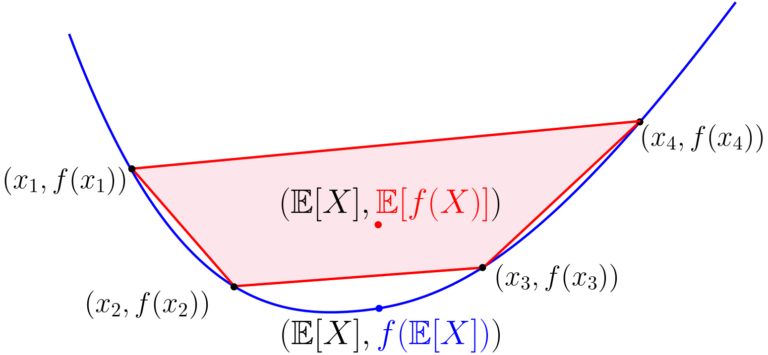
\includegraphics[scale=0.35]{./img/em/jensens_inequality}
		\caption{Visualisierung der Ungleichung von Jensen.}
	\end{figure}
\end{frame}


% SUBSECTION: Herleitung des Expectation-Schritts
\subsection{Herleitung des Expectation-Schritts}

% Bestimmung der unteren Schranke
\begin{frame}{Bestimmung der unteren Schranke}{}
	\begin{itemize}
		\item Im Folgenden konstruieren wir die oben erwähnte untere Schranke für $\ln p(\bX \param \btheta)$.
		\item Hierzu führen wir die Verteilung $q$ über $\bZ$ mit $q(\bZ) \ne 0$ ein und erhalten
		\begin{align*}
			\ln p(\bX \param \btheta)
				&= \ln \sum_{\bZ} p(\bX, \bZ \param \btheta)
					= \ln \sum_{\bZ} q(\bZ) \cdot \frac{p(\bX, \bZ \param \btheta)}{q(\bZ)}
		\\[2mm]
				&= \ln \E_{\bZ \sim q(\bZ)}\left[ \frac{p(\bX, \bZ \param \btheta)}{q(\bZ)} \right]
		\\[2mm]
				&\ge \E_{\bZ \sim q(\bZ)} \left[ \ln \frac{p(\bX, \bZ \param \btheta)}{q(\bZ)} \right] \eqqcolon \sL(q, \btheta).
		\end{align*}
		\item Für die Abschätzung im letzten Schritt haben wir die \keyword{Ungleichung von Jensen}, Satz \ref{th:em-jensen}, mit
			$f(x) \coloneqq \ln(x)$ \textit{(der Logarithmus ist strikt konkav)} und $X \coloneqq \frac{p(\bX, \bZ \param \btheta)}{q(\bZ)}$ benutzt.
	\end{itemize}
\end{frame}


% Bestimmung der unteren Schranke (Forts.)
\begin{frame}{Bestimmung der unteren Schranke (Forts.)}{}
	\begin{itemize}
		\item Die hergeleitete Ungleichung lässt sich mit den Logarithmengesetzen und der Linearität des Erwartungswerts umschreiben zu
		\begin{equation} \label{eq:em-lower-bound}
			\ln p(\bX \param \btheta) \ge \underbrace{
				\E_{\bZ \sim q(\bZ)}\left[ \ln p(\bX, \bZ \param \btheta) \right]
			}_{\substack{\text{\keyword{Erwartete vollständige}} \\ \text{\keyword{Log-Likelihood}}}} - 
			\underbrace{
				\E_{\bZ \sim q(\bZ)}\left[ \ln q(\bZ) \right]
			}_{\text{\keyword{Entropie} von $q$}}.
		\end{equation}
		\item Die untere Schranke hängt von der Dichte $q$ ab, die wir noch bestimmen müsssen.
		\item Wir möchten $q$ so wählen, dass für das aktuelle $\btheta$ in \eqref{eq:em-lower-bound} Gleichheit gilt.
		\item Die Ungleichung von Jensen, Satz \ref{th:em-jensen}, gilt mit Gleichheit, falls
		\begin{equation*}
			\frac{p(\bX, \bZ \param \btheta)}{q(\bZ)} = \const.
		\end{equation*}
	\end{itemize}
\end{frame}


% Bestimmung der unteren Schranke (Forts.)
\begin{frame}{Bestimmung der unteren Schranke (Forts.)}{}
	\begin{itemize}
		\item Wegen der vorausgehenden Überlegungen müssen wir also $q(\bZ) \propto p(\bX, \bZ \param \btheta)$ wählen. \\
			Das Symbol $\propto$ bedeutet \textit{'proportional zu'}.
		\item Daraus erhalten wir (da $q$ normiert sein muss)
		\begin{align*}
			q(\bZ)
				&= \frac{p(\bX, \bZ \param \btheta)}{\sum_{\bZtilde} p(\bX, \bZtilde \param \btheta)}
					= \frac{p(\bX, \bZ \param \btheta)}{p(\bX \param \btheta)}
		\\[2mm]
				&= p(\bZ \mid \bX \param \btheta).
		\end{align*}
		\item \textbf{Ergebnis:} Für $q$ benutzen wir die Posterior-Verteilung von $\bZ$ gegeben $\bX$.
		\item Dies setzen wir in \eqref{eq:em-lower-bound} ein und erhalten die Identität
		\begin{equation*}
			\ln p(\bX \param \btheta) = \E_{\bZ \sim p(\bZ\,\mid\,\bX \param \btheta)}\left[ \ln p(\bX, \bZ \param \btheta) \right]
				- \E_{\bZ \sim p(\bZ\,\mid\,\bX \param \btheta)}\left[ \ln p(\bZ \mid \bX \param \btheta) \right].
		\end{equation*}
	\end{itemize}
\end{frame}


% SUBSECTION: Herleitung des Maximization-Schritts
\subsection{Herleitung des Maximization-Schritts}

% Maximierung der unteren Schranke
\begin{frame}{Maximierung der unteren Schranke}{}
	\begin{itemize}
		\item Zu Beginn einer jeden EM-Iteration verfügen wir über den Parametervektor $\bthetaOld$, mit dem wir im E-Schritt
			die untere Schranke konstruieren.
		\item Hierbei wählen wir $q(\bZ) \coloneqq p\bigl( \bZ \mid \bX \param \bthetaOld \bigr)$.
		\item Als untere Schranke erhalten wir damit
		\begin{align*}
			\ln p(\bX \param \btheta)
				&\ge \E_{\bZ \sim p(\bZ\,\mid\,\bX \param \bthetaOld)}\left[ \ln p\bigl( \bX, \bZ \param \btheta \bigr) \right]
					- \E_{\bZ \sim p(\bZ\,\mid\,\bX \param \bthetaOld)}\left[ \ln p\bigl( \bZ \mid \bX \param \bthetaOld \bigr) \right]
		\\[2mm]
				&= Q\bigl( \btheta, \bthetaOld \bigr) + H\bigl( \bthetaOld, \bthetaOld \bigr)
		\\[2mm]
				&= Q\bigl( \btheta, \bthetaOld \bigr) + \const,
		\end{align*}
			wobei $Q$ der erste Erwartungswert und $H$ der negierte zweite Erwartungswert ist.
		\item Die Funktion $H\bigl( \bthetaOld, \bthetaOld \bigr)$ ist die \keyword{Entropie} von $q$ unter $\bthetaOld$.
	\end{itemize}
\end{frame}


% Maximierung der unteren Schranke (Forts.)
\begin{frame}{Maximierung der unteren Schranke (Forts.)}{}
	\begin{itemize}
		\item Da die Entropie $H\bigl( \bthetaOld, \bthetaOld \bigr)$ bezüglich $\btheta$ konstant ist, ist der im M-Schritt zu maximierende
			Ausdruck durch $Q\bigl( \btheta, \bthetaOld \bigr)$ gegeben.
		\item Der M-Schritt hat damit also die Gestalt
		\begin{equation} \label{eq:em-m-step}
			\bthetaNew \coloneqq \argmax_{\btheta} Q\bigl( \btheta, \bthetaOld \bigr).
		\end{equation}
		\item Weiter unten beweisen wir noch, dass tatsächlich $p\bigl(\bX \mid \bthetaNew \bigr) \ge p\bigl(\bX \mid \bthetaOld \bigr)$ gilt,
			dass also eine Iteration des EM-Verfahrens die Log-Likelihood tatsächlich erhöht.
		\item Zunächst fassen wir den EM-Algorithmus übersichtlich zusammen.
	\end{itemize}
\end{frame}


% SUBSECTION: EM-Algorithmus und Konvergenz
\subsection{EM-Algorithmus und Konvergenz}

% EM-Algorithmus
\begin{frame}{EM-Algorithmus}{}
	\begin{myalg}
		\begin{enumerate}
			\item Initialisiere $\bthetaOld$ \textit{(entweder zufällig oder mit Vorwissen)}.
			\item \textbf{E-Schritt:} Bestimme die untere Schranke
			\begin{equation*}
				Q\bigl( \btheta, \bthetaOld \bigr) \coloneqq \E_{\bZ \sim p(\bZ\,\mid\,\bX \param \bthetaOld)}\left[ \ln p(\bX, \bZ \param \btheta) \right].
			\end{equation*}
			\item \textbf{M-Schritt:} Maximiere die untere Schranke und berechne
			\begin{equation*}
				\bthetaNew \coloneqq \argmax_{\btheta} Q\bigl( \btheta, \bthetaOld \bigr).
			\end{equation*}
			\item Falls noch keine Konvergenz vorliegt, gehe zurück zu Schritt 2 und setze $\bthetaOld \coloneqq \bthetaNew$.
			\item Ansonsten gebe $\bthetaNew$ zurück.
		\end{enumerate}
	\end{myalg}
\end{frame}


% Konvergenz des EM-Algorithmus
\begin{frame}{Konvergenz des EM-Algorithmus}{}
	\begin{itemize}
		\item Zum Abschluss beweisen wir noch die Konvergenz des EM-Algorithmus
		\begin{align*}
			\ln p\bigl( \bX \param \bthetaNew \bigr)
				&\ge \sum_{\bZ} p\bigl( \bZ \mid \bX \param \bthetaOld \bigr)
					\ln \frac{p\bigl( \bX, \bZ \param \bthetaNew \bigr)}{p\bigl( \bZ \mid \bX \param \bthetaOld \bigr)}
		\\[2mm]
				&\ge \sum_{\bZ} p\bigl( \bZ \mid \bX \param \bthetaOld \bigr)
					\ln \frac{p\bigl( \bX, \bZ \param \bthetaOld \bigr)}{p\bigl( \bZ \mid \bX \param \bthetaOld \bigr)}
					= \ln p\bigl( \bX \param \bthetaOld \bigr).
		\end{align*}
		\item Die erste Ungleichung gilt hierbei aufgrund der Definition der unteren Schranke.
		\item Die zweite Ungleichung gilt, weil $\bthetaNew$ so gewählt wurde, dass es die untere Schranke maximiert.
		\item Die letzte Gleichheit gilt, da die untere Schranke bzgl. $\bthetaOld$ die Log-Likelihood in $\bthetaOld$ berührt.
	\end{itemize}
	
	\begin{boxGray}
		\textbf{Bemerkung:} Allerdings kann das Verfahren in lokalen Maxima hängen bleiben!
	\end{boxGray}
\end{frame}


% Visualisierung: EM-Algorithmus
\begin{frame}{Visualisierung: EM-Algorithmus}{}
	\begin{figure}
		\centering
		
\includegraphics[scale=0.75]{./img/em/em_visual}
		\caption{Veranschaulichung des EM-Algorithmus. Siehe \cite{Bishop2024}, Seite 488.}
	\end{figure}
\end{frame}


% SUBSECTION: Evidence-Lower-Bound und Kullback-Leibler Divergenz
\subsection{Evidence-Lower-Bound und Kullback-Leibler Divergenz}


% Aufgabe: EM für Probleme mit fehlenden Daten
\begin{frame}{Aufgabe: EM für Probleme mit fehlenden Daten}{}
	\begin{mytask}[task:em-missing-data]
		Das EM-Verfahren kann auch für Schätzprobleme benutzt werden, falls einzelne Werte im Datensatz fehlen.
		Eine Voraussetzung ist jedoch, dass das Fehlen der Daten zufällig ist und nicht systematisch.
		
		Man nehme an...
	\end{mytask}
\end{frame}


% Evidence Lower Bound (ELBO)
\begin{frame}{Evidence Lower Bound (ELBO)}{}
	\begin{itemize}
		\item Wir geben noch eine andere Sicht auf den EM-Algorithmus.
		\item Hierzu stellen wir fest, dass wir die Log-Likelihood $\ln p(\bX \param \btheta)$ folgendermaßen zerlegen können
		\begin{equation} \label{eq:em-decomposition-incomplete-log-likelihood}
			\ln p(\bX \param \btheta) = \sL(q, \btheta) + \KL(q \parallel p).
		\end{equation}
		\item Dabei ist:
		\begin{itemize}
			\item $\sL(q, \btheta)$ die \keyword{Evidence Lower Bound (ELBO)} oder auch \keyword{Variational Lower Bound}
			\begin{equation} \label{eq:em-elbo}
				\sL(q, \btheta)
					\coloneqq \sum_{\bZ} q(\bZ) \ln \frac{p(\bX, \bZ \param \btheta)}{q(\bZ)}
					= \sum_{\bZ} q(\bZ) \cdot \bigl[ \ln p(\bX, \bZ \param \btheta) - \ln q(\bZ) \bigr].
			\end{equation}
			\item $\KL(q \parallel p)$ die \keyword{Kullback-Leibler Divergenz} zwischen $q(\bZ)$ und $p(\bZ \mid \bX \param \btheta)$
			\begin{equation} \label{eq:em-kl-div}
				\KL(q \parallel p)
					\coloneqq -\sum_{\bZ} q(\bZ) \ln \frac{p(\bZ \mid \bX \param \btheta)}{q(\bZ)}
					= -\sum_{\bZ} q(\bZ) \cdot \bigl[ \ln p(\bZ \mid \bX \param \btheta) - \ln q(\bZ) \bigr].
			\end{equation}
		\end{itemize}
	\end{itemize}
\end{frame}


% Beweis der Zerlegung \eqref{eq:em-decomposition-incomplete-log-likelihood}
\begin{frame}{Beweis der Zerlegung \eqref{eq:em-decomposition-incomplete-log-likelihood}}{}
	\begin{myproof}
		Wir beweisen die Zerlegung \eqref{eq:em-decomposition-incomplete-log-likelihood}.
		Hierzu wenden wir die Kettenregel für Wahrscheinlichkeiten auf $p(\bX, \bZ \param \btheta)$ an.
		Wir erhalten $p(\bX, \bZ \param \btheta) = p(\bZ \mid \bX \param \btheta) \cdot p(\bX \param \btheta)$.
		Anwendung des Logarithmus ergibt $$\ln p(\bX, \bZ \param \btheta) = \ln p(\bZ \mid \bX \param \btheta) + \ln p(\bX \param \btheta).$$
		Dies setzen wir in die Evidence Lower Bound \eqref{eq:em-elbo} ein und erhalten
		\begin{align*}
			\sL(q, \btheta)
				&= \sum_{\bZ} q(\bZ) \cdot \bigl[ \ln p(\bX, \bZ \param \btheta) - \ln q(\bZ) \bigr]
		\\[2mm]
				&= \sum_{\bZ} q(\bZ) \cdot \bigl[ \ln p(\bZ \mid \bX \param \btheta) + \ln p(\bX \param \btheta) - \ln q(\bZ) \bigr].
		\end{align*}
		Damit ergibt sich schließlich mit \eqref{eq:em-kl-div} und wegen $\sum_{\bZ} q(\bZ) = 1$
		\begin{align*}
			\sL(q, \btheta) + \KL(q \parallel p)
				&= \sum_{\bZ} q(\bZ) \cdot \bigl[ \ln p(\bZ \mid \bX \param \btheta) + \ln p(\bX \param \btheta) - \ln q(\bZ) \bigr]
					- \sum_{\bZ} q(\bZ) \cdot \bigl[ \ln p(\bZ \mid \bX \param \btheta) - \ln q(\bZ) \bigr]
		\\[2mm]
				&= \sum_{\bZ} q(\bZ) \cdot \ln p(\bX \param \btheta) = \ln p(\bX \param \btheta) \cdot \sum_{\bZ} q(\bZ) = \ln p(\bX \param \btheta).
		\end{align*}
	\end{myproof}
\end{frame}


% Kullback-Leibler Divergenz
\begin{frame}{Kullback-Leibler Divergenz}{}
	\textbf{Eigenschaften der Kullback-Leibler Divergenz:}
	
	\begin{boxGray}
		Für alle Wahrscheinlichkeitsverteilungen $q$ und $p$ gelten die folgenden Eigenschaften.

		\begin{enumerate}
			\item \textbf{Nicht-Negativität:}
			\begin{equation} \label{eq:em-kl-non-neg}
				\KL(q \parallel p) \ge 0
			\end{equation}
			\item \textbf{Identität:}
			\begin{equation} \label{eq:em-kl-ident}
				\KL(q \parallel p) = 0 \quad\Longleftrightarrow\quad q = p.
			\end{equation}
			\item Die Kullback-Leibler Divergenz ist \textbf{nicht symmetrisch} und damit keine Metrik. Es ist also im Allgemeinen
			\begin{equation*}
				\KL(q \parallel p) \ne \KL(p \parallel q).
			\end{equation*}
		\end{enumerate}
	\end{boxGray}
\end{frame}


% Kullback-Leibler Divergenz (Forts.)
\begin{frame}{Kullback-Leibler Divergenz (Forts.)}{}
	\begin{itemize}
		\item Aus \eqref{eq:em-kl-div} ist ersichtlich, dass $\KL(q \parallel p)$ die Kullback-Leibler Divergenz zwischen
			der Verteilung $q(\bZ)$ und der Posterior-Verteilung $p(\bZ \mid \bX \param \btheta)$ von $\bZ$ ist.
		\item Aus der Zerlegung \eqref{eq:em-decomposition-incomplete-log-likelihood} folgt mit der Nichtnegativität \eqref{eq:em-kl-non-neg}
			der Kullback-Leibler Divergenz
		\begin{equation*}
			\sL(q, \btheta) \le p(\bX \param \btheta).
		\end{equation*}
		\item $\sL(q, \btheta)$ ist also eine untere Schranke für $p(\bX \param \btheta)$.
	\end{itemize}
\end{frame}


% Visualisierung: Zerlegung der Log-Likelihood
\begin{frame}{Visualisierung: Zerlegung der Log-Likelihood}{}
	\begin{figure}
		\centering
		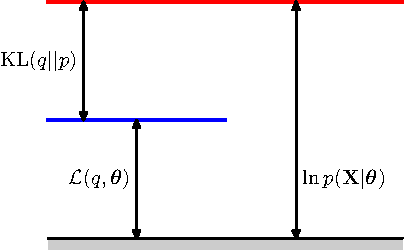
\includegraphics[scale=1.00]{./img/em/em_decomposition_log_likelihood}
		\caption{Veranschaulichung der Zerlegung \eqref{eq:em-decomposition-incomplete-log-likelihood}. Siehe \cite{Bishop2024}, Seite 486.}
	\end{figure}
\end{frame}


% Eine andere Sicht auf den E-Schritt
\begin{frame}{Eine andere Sicht auf den E-Schritt}{}
	\begin{itemize}
		\item Mit dieser Vorarbeit können wir nun die alternative Herleitung des EM-Algorithmus durchführen.
		\item Im \keyword{E-Schritt} wird die untere Schranke $\sL\bigl( q, \bthetaOld \bigr)$ bezüglich $q(\bZ)$
			bei gegebenem $\bthetaOld$ maximiert, sodass die untere Schranke die eigentliche Zielfunktion
			$\ln p(\bX \param \btheta)$ in $\bthetaOld$ berührt.
		\item Da $p\bigl( \bX \param \bthetaOld \bigr)$ nicht von $q(\bZ)$ abhängt, folgt aus der Maximierung von $\sL\bigl( q, \bthetaOld \bigr)$,
			dass $\KL(q \parallel p) = 0$ gelten muss.
		\item Damit $\KL(q \parallel p) = 0$ gilt, muss wegen \eqref{eq:em-kl-ident} für $q(\bZ)$ gelten
		\begin{equation*}
			q(\bZ) = p\bigl( \bZ \mid \bX \param \bthetaOld \bigr).
		\end{equation*}
		\item Das heißt, nach dem E-Schritt gilt
		\begin{equation*}
			\sL\bigl( q, \bthetaOld \bigr) = \ln p\bigl( \bX \param \bthetaOld \bigr).
		\end{equation*}
	\end{itemize}
\end{frame}


% Visualisierung: E-Schritt
\begin{frame}{Visualisierung: E-Schritt}{}
	\begin{figure}
		\centering
		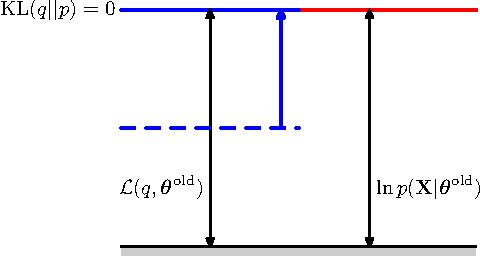
\includegraphics[scale=1.00]{./img/em/em_e_step}
		\caption{Veranschaulichung des E-Schritts. Siehe \cite{Bishop2024}, Seite 486.}
	\end{figure}
\end{frame}


% Eine andere Sicht auf den M-Schritt
\begin{frame}{Eine andere Sicht auf den M-Schritt}{}
	\begin{itemize}
		\item Im darauffolgenden \keyword{M-Schritt} halten wir nun die Verteilung $q(\bZ)$ fest und maximieren die untere Schranke $\sL(q, \btheta)$
			bezüglich $\btheta$.
		\item Hierdurch erhalten wir die neuen Parameter $\bthetaNew$, die letztendlich zu einer höheren
			Log-Likelihood $p(\bX \param \btheta)$ führen.
		\item Setzen wir $q(\bZ) = p\bigl( \bZ \mid \bX \param \bthetaOld \bigr)$ in die Definition der unteren Schranke \eqref{eq:em-elbo} ein,
			so erhalten wir
		\begin{align*}
			\sL(q, \btheta)
				&= \sum_{\bZ} p\bigl( \bZ \mid \bX \param \bthetaOld \bigr) \ln p(\bX, \bZ \param \btheta)
					- \sum_{\bZ} p\bigl( \bZ \mid \bX \param \bthetaOld \bigr) \ln p\bigl( \bZ \mid \bX \param \bthetaOld \bigr)
		\\[2mm]
				&= Q\bigl( \btheta, \bthetaOld \bigr) + \const,
		\end{align*}
		wobei $\const$ wieder die Entropie von $q$ ist.
	\end{itemize}
\end{frame}


% Eine andere Sicht auf den M-Schritt (Forts.)
\begin{frame}{Eine andere Sicht auf den M-Schritt (Forts.)}{}
	\begin{itemize}
		\item Um die gegebene untere Schranke zu maximieren, müssen wir also die Funktion $Q\bigl( \btheta, \bthetaOld \bigr)$ maximieren,
			wobei $Q$ die \keyword{erwartete vollständige Log-Likelihood} ist.
		\item Damit nimmt der M-Schritt dieselbe Form wie in \eqref{eq:em-m-step} an
		\begin{equation*}
			\bthetaNew \coloneqq \argmax_{\btheta} Q\bigl( \btheta, \bthetaOld \bigr).
		\end{equation*}
		\item Weil die Verteilung $q$ im vorhergehenden E-Schritt mit den alten Parametern $\bthetaOld$ bestimmt wurde und diese
			für den gesamten M-Schritt fixiert wird, gilt
		\begin{equation*}
			q(\bZ) = p\bigl( \bZ \mid \bX \param \bthetaOld \bigr) \ne p\bigl( \bZ \mid \bX \param \bthetaNew \bigr),
		\end{equation*}
			sodass die Kullback-Leibler Divergenz zwischen diesen beiden Verteilung größer als 0 ist.
		\item Im folgenden E-Schritt setzen wir dann $q(\bZ) \coloneqq p\bigl( \bZ \mid \bX \param \bthetaNew \bigr)$ und iterieren weiter.
	\end{itemize}
\end{frame}


% Visualisierung: M-Schritt
\begin{frame}{Visualisierung: M-Schritt}{}
	\begin{figure}
		\centering
		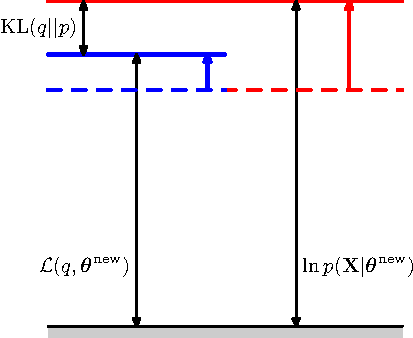
\includegraphics[scale=0.90]{./img/em/em_m_step}
		\caption{Veranschaulichung des M-Schritts. Siehe \cite{Bishop2024}, Seite 487.}
	\end{figure}
\end{frame}


% SUBSECTION: Anwendung auf Gaussian Mixture Models
\subsection{Anwendung auf Gaussian Mixture Models}

% Gaussian Mixture Models und EM
\begin{frame}{Gaussian Mixture Models und EM}{}
	\begin{itemize}
		\item Wir wenden das allgemeine EM-Framework nun auf GMMs an.
		\item Im E-Schritt benötigen wir die Aposteriori-Verteilung $p(\bZ \mid \bX \param \btheta)$ der latenten Variablen, wobei
			$\btheta \coloneqq \bigl( \bpi, \bmu, \bSigma \bigr) \coloneqq
			\bigl( \pi_1, \ldots, \pi_K, \bmu_1, \ldots, \bmu_K, \bSigma_1, \ldots, \bSigma_K \bigr)$ ist.
		\item Diese können wir mit \eqref{eq:gmm-marginal-z}, \eqref{eq:gmm-x-given-z} und dem Satz von Bayes bestimmen zu
		\begin{equation*}
			p(\bZ \mid \bX \param \btheta)
				\propto \prod_{n=1}^N \prod_{k=1}^K \bigl[ \pi_k \cdot \norm(\bx_n \param \bmu_k, \bSigma_k) \bigr]^{z_{nk}}.
		\end{equation*}
		\item Als nächstes stellen wir die erwartete vollständige Log-Likelihood auf, wobei der Erwartungswert bezüglich der
			Aposteriori-Verteilung $p(\bZ \mid \bX \param \btheta)$ zu berechnen ist.
		\item Dazu benötigen wir allerdings noch ein Zwischenergebnis, das wir auf der nächsten Folie bereitstellen.
	\end{itemize}
\end{frame}


% Gaussian Mixture Models und EM (Forts.)
\begin{frame}{Gaussian Mixture Models und EM (Forts.)}{}
	\begin{itemize}
		\item Es gilt der Zusammenhang
		\begin{equation} \label{eq:gmm-latent-var-expected-value}
			\begin{aligned}
				\E_{\bZ \sim p(\bZ \mid \bX \param \btheta)}[z_{nk}]
					&= \frac{
						\displaystyle\sum_{\bz_n} z_{nk} \prod_{k'=1}^K \bigl[ \pi_{k'} \cdot \norm(\bx_n \param \bmu_{k'}, \bSigma_{k'}) \bigr]^{z_{nk'}}
					}{
						\displaystyle\sum_{\bz_n} \prod_{j=1}^K \bigl[ \pi_j \cdot \norm(\bx_n \param \bmu_j, \bSigma_j) \bigr]^{z_{nj}}
					}
			\\[2mm]
					&= \frac{\pi_k \cdot \norm(\bx_n \param \bmu_k, \bSigma_k)}{\displaystyle\sum_{j=1}^K \pi_j \cdot \norm(\bx_n \param \bmu_j, \bSigma_j)}
						= \gamma(z_{nk}).
			\end{aligned}
		\end{equation}
		\item Der Erwartungswert der Indikator-Variablen $z_{nk}$ unter der Aposteriori-Verteilung von $\bZ$
			ergibt sich also gerade als die jeweilige Responsibility $\gamma(z_{nk})$.
	\end{itemize}
\end{frame}


% Gaussian Mixture Models und EM (Forts.)
\begin{frame}{Gaussian Mixture Models und EM (Forts.)}{}
	Hiermit können wir nun die \keyword{erwartete vollständige Log-Likelihood} (Funktion $Q$) aufstellen
	\begin{equation} \label{eq:gmm-expected-complete-log-likelihood}
		\begin{aligned}
			\E_{\bZ \sim p(\bZ \mid \bX \param \btheta)}\bigl[ \ln p(\bX, \bZ \param \btheta) \bigr]
				&= \E\left[
					\ln \prod_{n=1}^N \prod_{k=1}^K \pi_k^{z_{nk}} \cdot \norm(\bx_n \param \bmu_k, \bSigma_k)^{z_{nk}}
				\right]
		\\[2mm]
				&= \E\left[
					\sum_{n=1}^N \sum_{k=1}^K z_{nk} \cdot \bigl\{ \ln \pi_k + \ln \norm(\bx_n \param \bmu_k, \bSigma_k) \bigr\}
				\right]
				&& \rem{Logarithmengesetze.}
		\\[2mm]
				&= \sum_{n=1}^N \sum_{k=1}^K \E[z_{nk}] \cdot \bigl\{ \ln \pi_k + \ln \norm(\bx_n \param \bmu_k, \bSigma_k) \bigr\}
				&& \rem{Linearität von $\E$.}
		\\[2mm]
				&= \sum_{n=1}^N \sum_{k=1}^K \gamma(z_{nk}) \cdot \bigl\{ \ln \pi_k + \ln \norm(\bx_n \param \bmu_k, \bSigma_k) \bigr\}
				&& \rem{Anwendung von \eqref{eq:gmm-latent-var-expected-value}}.
		\end{aligned}
	\end{equation}
\end{frame}


% Gaussian Mixture Models und EM (Forts.)
\begin{frame}{Gaussian Mixture Models und EM (Forts.)}{}
	\begin{itemize}
		\item Die Funktion \eqref{eq:gmm-expected-complete-log-likelihood} müssen wir nun im M-Schritt bezüglich der Parameter maximieren.
		\item \textbf{Beispielhaft:} Gradient bezüglich $\bmu_k$
		\begin{align*}
			\frac{\partial}{\partial \bmu_k} \sum_{n=1}^N \sum_{j=1}^K \gamma(z_{nj}) \cdot
				\bigl\{ \ln \pi_j + \ln \norm(\bx_n \param \bmu_j, \bSigma_j) \bigr\}
			&= \sum_{n=1}^N \gamma(z_{nk}) \cdot \frac{\partial}{\partial \bmu_k} \ln \norm(\bx_n \param \bmu_k, \bSigma_k)
		\\[2mm]
			&= \sum_{n=1}^N \gamma(z_{nk}) \cdot \frac{\norm(\bx_n \param \bmu_k, \bSigma_k)}{\norm(\bx_n \param \bmu_k, \bSigma_k)}
				\cdot \bSigma_k^{-1} (\bx_n - \bmu_k)
		\\[2mm]
			&= \sum_{n=1}^N \gamma(z_{nk}) \cdot \bSigma_k^{-1} (\bx_n - \bmu_k).
		\end{align*}
		\item Vergleiche hierzu die Herleitung in \eqref{eq:gmm-grad-means}.
	\end{itemize}
\end{frame}


% Gaussian Mixture Models und EM (Forts.)
\begin{frame}{Gaussian Mixture Models und EM (Forts.)}{}
	\begin{itemize}
		\item Nullsetzen und Auflösen nach $\bmu_k$ ergibt $$\bmu_k = \frac{1}{N_k} \sum_{n=1}^N \gamma(z_{nk}) \cdot \bx_n.$$
		\item Dies hat dieselbe Form wie \eqref{eq:gmm-update-means}.
		\item Die anderen Formeln ergeben sich analog.
	\end{itemize}
\end{frame}